\documentclass[%
pdf,
%nocolorBG,
colorBG,
slideColor,
%slideBW,
%draft,
%frames
%azure
%contemporain
%nuancegris
%troispoints
%lignesbleues
%darkblue
%alienglow
%autumn
]{prosper}
\usepackage{pifont, amsmath, multicol}
%\usepackage{floatflt, wrapfig,subfigure}
%\usepackage{wrapfig}
%\usepackage{floatflt}
\usepackage{color}
\usepackage{epsfig}
\usepackage{pifont}
%\usepackage[francais]{babel}
\usepackage[T1]{fontenc}
\usepackage[latin1]{inputenc}
\input{emlines.sty}
%\def«{\og\ignorespaces}%
%\def»{{\fg}}%
\newcommand{\spacer}{\rule[-3mm]{0mm}{8mm}}

\newcommand{\RR}{\ensuremath{\mathbb{R}}}
\newcommand{\NN}{\ensuremath{\mathbb{N}}}
\newcommand{\QQ}{\ensuremath{\mathbb{Q}}}
\newcommand{\CC}{\ensuremath{\mathbb{C}}}
\newcommand{\ZZ}{\ensuremath{\mathbb{Z}}}
\newcommand{\TT}{\ensuremath{\mathbb{T}}}

\def\QuotS#1#2{\leavevmode\kern-.0em\raise.2ex\hbox{$#1$}\kern-.1em/\kern-.1em\lower.25ex\hbox{$#2$}}


\title{\Huge \textcolor{blue}{Polycycles and}\\[3mm]
\textcolor{blue}{their boundaries}}

\author{
\textcolor{red}{\Large Mathieu Dutour,}\\[2mm]
\textcolor{red}{\Large Michel Deza}\\[2mm]
\textcolor{red}{\Large and Mikhail Shtogrin}\\
}
\author{
\textcolor{red}{\Large Mathieu Dutour}\\[2mm]
\textcolor{red}{\large ENS/CNRS, Paris and Hebrew University, Jerusalem}\\[2mm]
\textcolor{red}{\Large Michel Deza}\\[2mm]
\textcolor{red}{\large ENS/CNRS, Paris and ISM, Tokyo}\\[2mm]
\textcolor{red}{\Large and Mikhail Shtogrin}\\[2mm]
\textcolor{red}{\large Steklov Institute, Moscow}
}


\slideCaption{}

\date{}



\begin{document}
\maketitle




\begin{slide}{}
\begin{center}
{\Huge 
\begin{tabular*}{7cm}{c}
\\[-0.5cm]
\textcolor{blue}{I. }\textcolor{red}{$(p,3)$-polycycles}
\end{tabular*}
}
\end{center}
\end{slide}



%$G$ of girth $p$ and maximal vertex-degree $s$, which admits
%a realization on the plane, such that:

\begin{slide}{Polycycles}
A finite \textcolor{red}{$(p,3)$-polycycle} is a plane $2$-connected finite graph, such that :
\begin{itemize}
\item all interior faces are (combinatorial) $p$-gons,
\item all interior vertices are of degree $3$,
\item all boundary vertices are of degree $2$ or $3$.
\end{itemize}

\begin{center}
\epsfig{file=Boundary/3_5_polycycle.eps, width=4cm}
\end{center}
%All polycycles considered have $s=3$ and are finite.

\end{slide}


\begin{slide}{Theorem}
The \textcolor{red}{skeleton} of a plane graph is the graph formed by its vertices and edges.
{\it

{\bf Theorem}

A $(p,3)$-polycycle is determined by its skeleton
with the exception of the Platonic solids, for which any of their faces can
play role of exterior one

}
%This theorem applies even if the skeleton is not $3$-connected.

\begin{center}
\epsfig{file=Boundary/3_5_polycycleWrongEmbedding.eps, width=4cm}\par
an unauthorized plane embedding
\end{center}


\end{slide}








\begin{slide}{$(3,3)$ and $(4,3)$-polycycles}
{\it\scriptsize

%{\bf Theorem}

(i) \textcolor{red}{Any $(3,3)$-polycycle} is one of the following $3$ cases:
\begin{center}
\epsfig{figure=Boundary/Possible3gonalPatchNOB.eps,width=6cm}
\end{center}

(ii) \textcolor{red}{Any $(4,3)$-polycycle} belongs to the following $3$ cases:
\begin{center}
\epsfig{figure=Boundary/DiscreteCase4gonalPatchNOB.eps,width=6cm}
\end{center}
\hspace{1cm}or belong to the following infinite family of $(4,3)$-polycycles:
\begin{center}
\epsfig{figure=Boundary/InfiniteSequenceNOB.eps,width=8cm}
\end{center}

}
So, those two cases are trivial.

\end{slide}














\begin{slide}{Boundary sequences}
%The symmetry group of a $(p,3)$-polycycle is an useful invariant but it is hard to compute.
\vspace{-2mm}
The \textcolor{red}{boundary sequence} is the sequence of degrees (2~or~3) of the vertices of the boundary.
\begin{center}
\begin{minipage}{5cm}
\centering
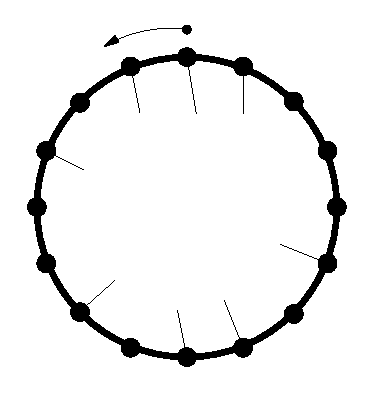
\epsfig{file=Boundary/TheExample.eps, width=2.1cm}
\end{minipage}
\begin{minipage}{5cm}
Associated sequence is
3323223233232223
\end{minipage}
\end{center}

\begin{itemize}
\item The boundary sequence is defined only up to action of $D_n$, i.e. the \textcolor{red}{dihedral group} of order $2n$ generated by cyclic shift and reflexion.
\item The invariant given by the boundary sequence is the smallest (by the lexicographic order) representative of the all possible boundary sequences.
\end{itemize}




\end{slide}
















\begin{slide}{Enumeration of $(p,3)$-polycycles}

\vspace{-2mm}
There exist a large litterature on enumeration of $(6,3)$-polycycles; they are called \textcolor{red}{benzenoids}.
\begin{center}
\begin{minipage}[t]{3.5cm}
\centering
\epsfxsize=9mm
\epsffile{Polycycle/ris-1bis-a.eps}\par
benzene $C_6H_6$
\end{minipage}
\begin{minipage}[t]{3.5cm}
\centering
\epsfxsize=15mm
\epsffile{Polycycle/ris-1bis-b.eps}\par
naphtalene $C_{10}H_8$
\end{minipage}
\begin{minipage}[t]{3.5cm}
\centering
\epsfxsize=15mm
\epsffile{Boundary/Azulene.eps}\par
azulene $C_{10}H_8$
\end{minipage}

\end{center}

Algorithm for enumerating $(p,3)$-polycycles with $n$ $p$-gons:
\begin{itemize}
\item Compute the list of all $p$-gonal patches with $n\hspace{-1mm}-\hspace{-1mm}1$ $p$-gons
\item Add a $p$-gon to it in all possible ways
\item Compute invariants like their smallest (by the lexicographic order) boundary sequence
\item Keep a list of nonisomorph representatives (we use here the program {\bf nauty} by Brendan Mc Kay)
\end{itemize}
\end{slide}







\begin{slide}{Enumeration of small $(5,3)$-polycycles}
%\vspace{-5mm}
\begin{center}
\begin{minipage}{58mm}
\centering
\epsfig{file=Boundary/FirstCase35poly1.eps, width=1cm}\par
$n=1$\\
\epsfig{file=Boundary/FirstCase35poly2.eps, width=2cm}\par
$n=2$\\[2mm]
{\scriptsize
\begin{tabular}{||c|c||c|c||c|c||}
\hline
$n$&     &$n$&        &$n$&\\
\hline
1  &1    &6  &18      &11 &1337\\
2  &1    &7  &35      &12 &3524\\
3  &2    &8  &87      &13 &9262\\
4  &4    &9  &206     &14 &24772\\
5  &7    &10 &527     &15 &66402\\
\hline
\end{tabular}
}
\end{minipage}
\begin{minipage}{45mm}
\centering
\epsfig{file=Boundary/FirstCase35poly3.eps, width=4cm}\par
$n=3$\\
\epsfig{file=Boundary/FirstCase35poly4.eps, width=5cm}\par
$n=4$\\
\end{minipage}
\end{center}


\end{slide}




\begin{slide}{Benzenoids of lattice type}

We say that a $(6,3)$-polycyle has \textcolor{red}{lattice type} if its skeleton is a partial subgraph of the skeleton of the partition of the plane into hexagons.
\begin{center}
\epsfig{figure=Boundary/LatticeHexagon.eps,height=1.9cm}
\end{center}
Such $(6,3)$-polycycles are uniquely defined by their boundary sequence.

{\scriptsize
M. Deza, P.W. Fowler, V.P. Grishukhin, {\em Allowed boundary sequences for fused polycyclic patches, and related algorithmic problems}, Journal of Chemical Information and Computer science {\bf 41-2} (2001) 300--308.
}


\end{slide}



















\begin{slide}{}
\begin{center}
{\Huge 
\begin{tabular*}{8cm}{c}
\\[-0.5cm]
\textcolor{blue}{II. }\textcolor{red}{$(p,3)$-polycycles}\\
\textcolor{red}{with}
\textcolor{red}{given boundary}
\end{tabular*}
}
\end{center}
\end{slide}




\overlays{2}{
\begin{slide}{The filling problem}
\fromSlide{1}{
\begin{itemize}
\item Does there exist $(p,3)$-polycycles with given boundary sequence?
\item If yes, is this $(p,3)$-polycycle unique?
\item Find an algorithm for solving those problems computationally.
\end{itemize}
Remind, that the cases $p=3$ or $4$ are trivial.

Let $p=5$; consider, for example, the sequence $23 23 23 23 23$
}%
\onlySlide*{1}{
\begin{center}
\epsfig{figure=Boundary/ExampleProblem.eps,height=3cm}
\end{center}
}%
\onlySlide*{2}{
\begin{center}
\epsfig{figure=Boundary/ExampleSolution.eps,height=3cm}
\end{center}
}%


\end{slide}
}














\begin{slide}{The case of $(5,3)$-polycycles}
\vspace{-3mm}
Two $(5,3)$-polycycles with the same boundary.


\begin{center}
\begin{minipage}{55mm}
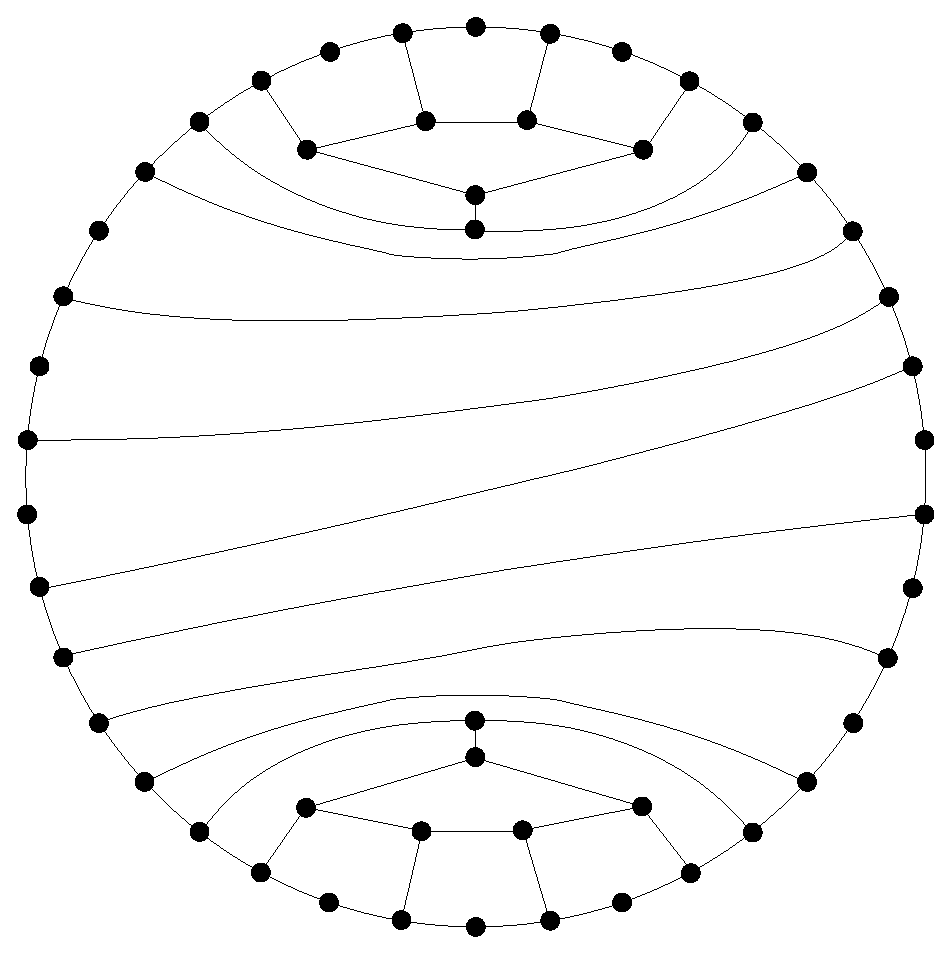
\epsfig{file=Boundary/HELICEN5gon.eps, width=5cm}
\end{minipage}
\begin{minipage}{55mm}
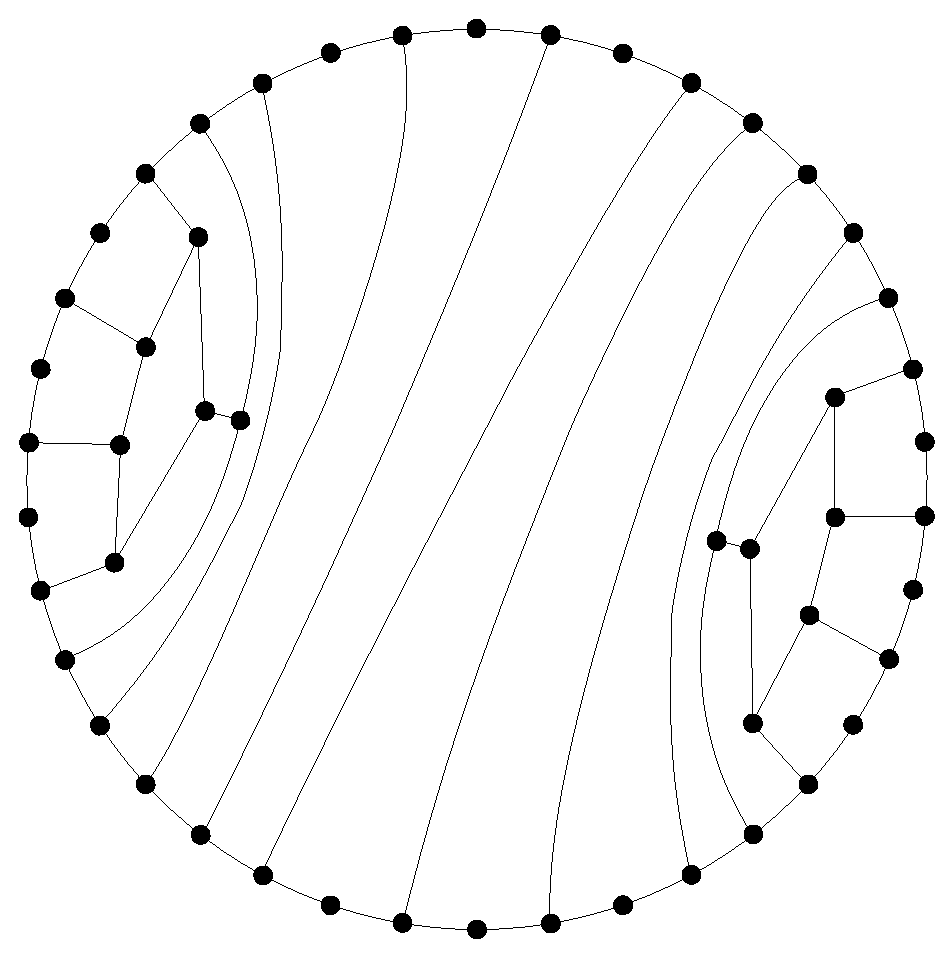
\epsfig{file=Boundary/HELICEN5gonSec.eps, width=5cm}
\end{minipage}
\textcolor{red}{Boundary sequence}: $12$, $26$ vertices of degree $2$, $3$, resp.\\
\textcolor{red}{Symmetry groups}: of boundary: $C_{2v}$, of polycycles: $C_2$.\\
\textcolor{red}{Fillings}: $20$ pentagons, $12$ interior points.
\end{center}




\end{slide}






\begin{slide}{The case of $(6,3)$-polycycles}
\vspace{-3mm}
Two $(6,3)$-polycycles with the same boundary.


\begin{center}
\begin{minipage}{55mm}
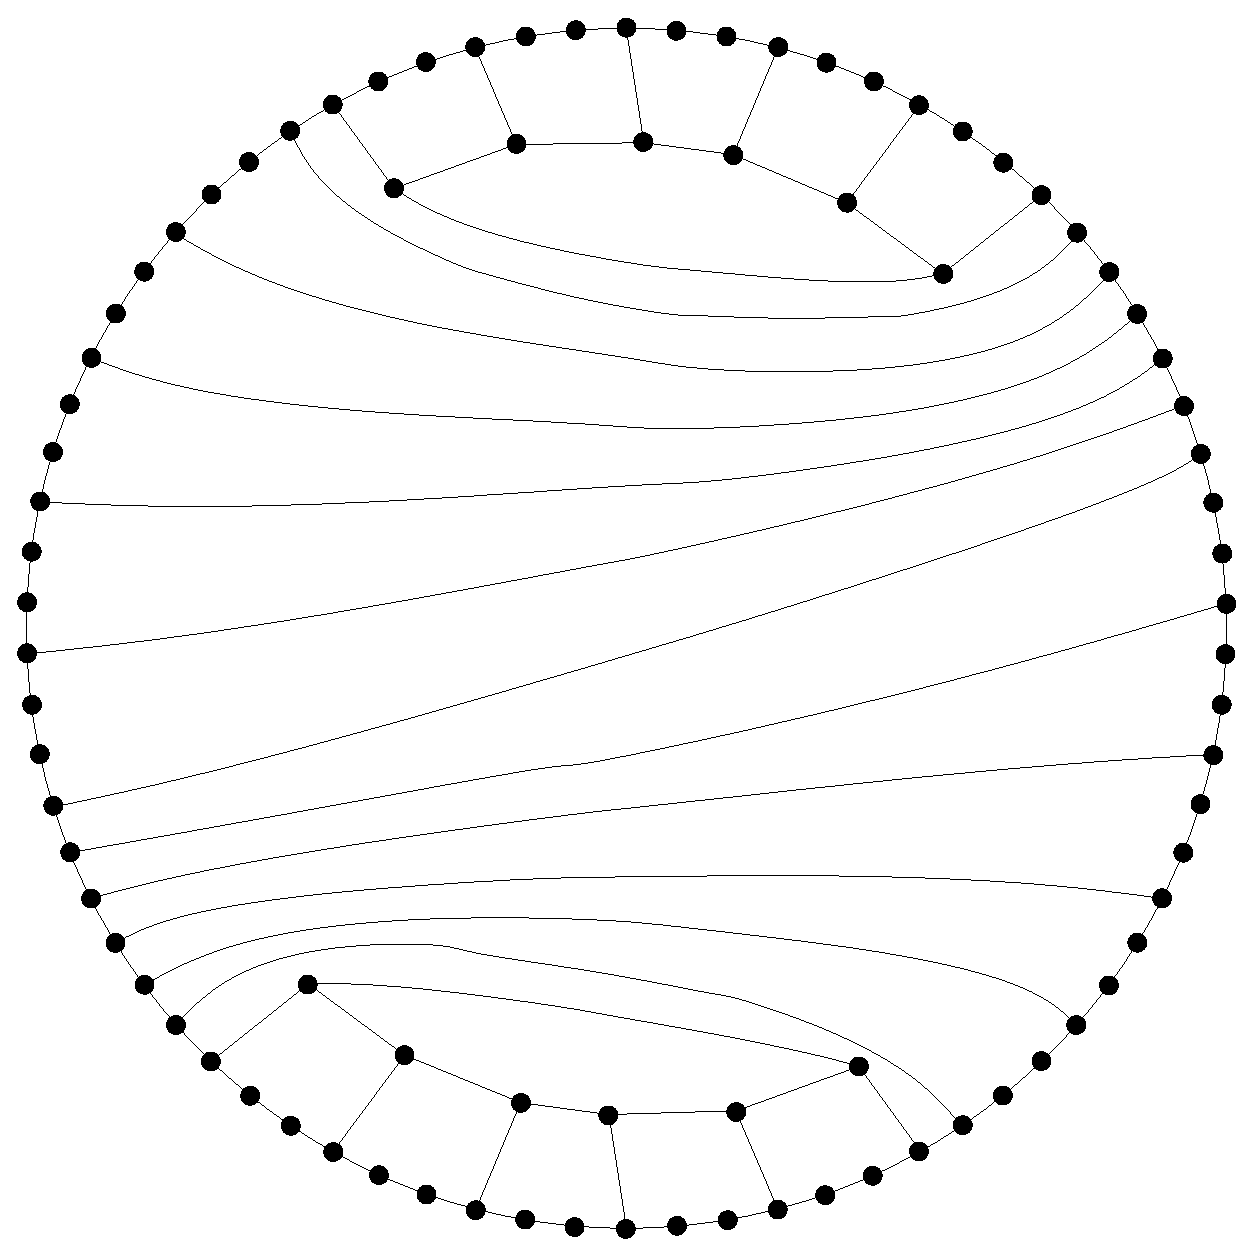
\epsfig{file=Boundary/HELICEN6gon.eps, width=5cm}
\end{minipage}
\begin{minipage}{55mm}
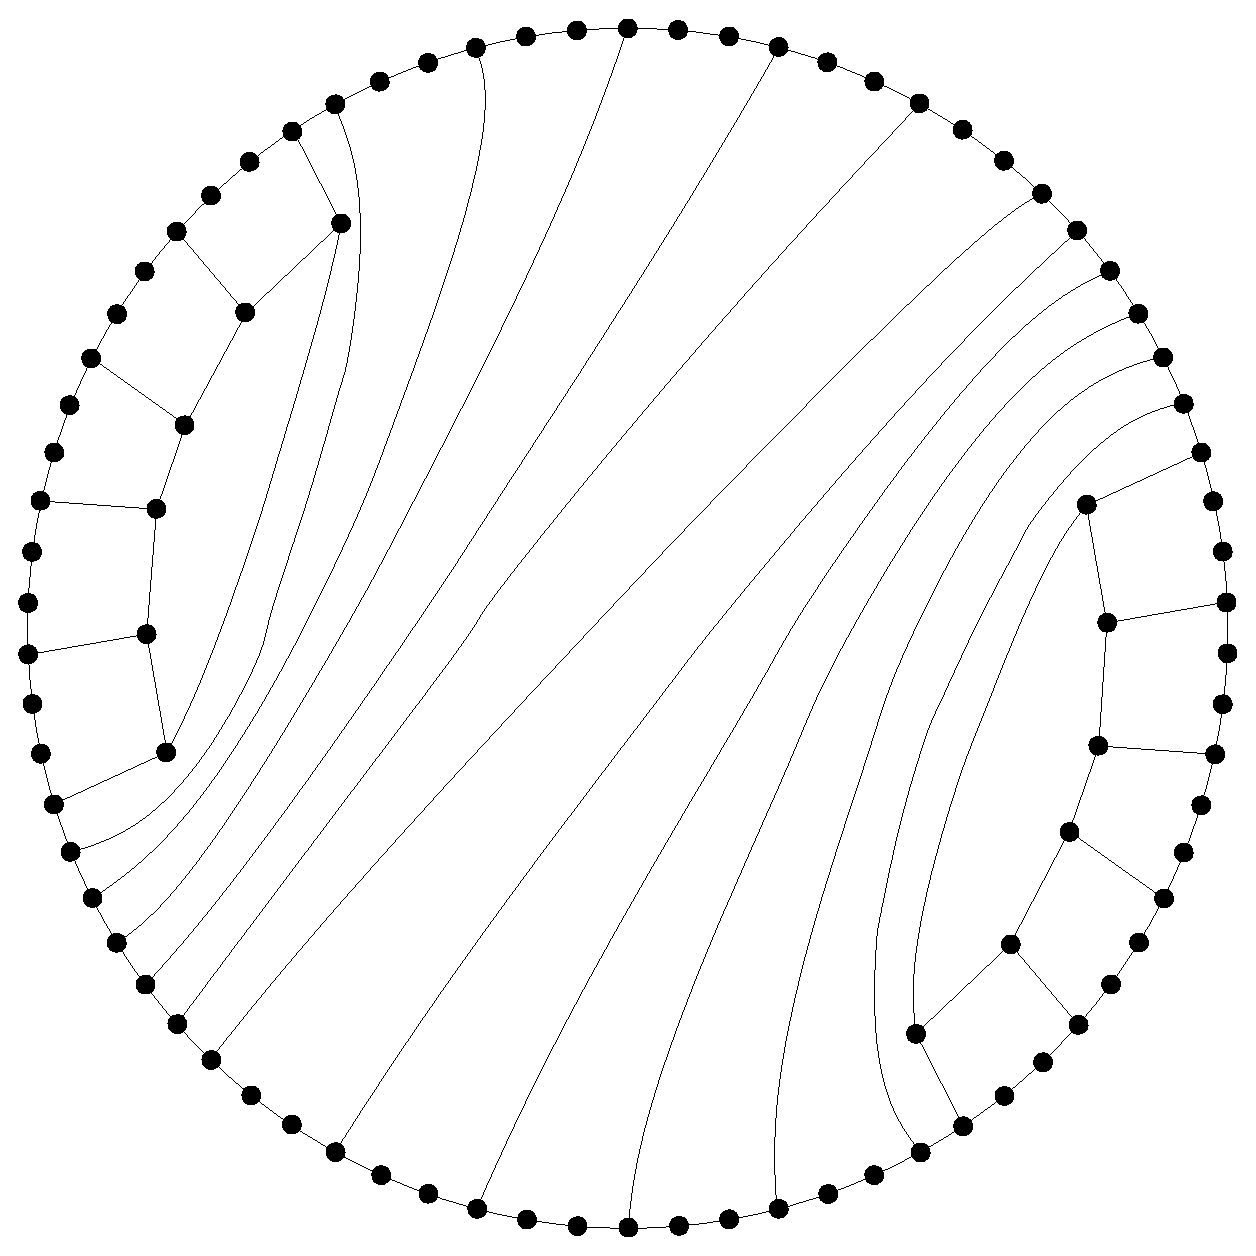
\epsfig{file=Boundary/HELICEN6gonSec.eps, width=5cm}
\end{minipage}
\textcolor{red}{Boundary sequence}: $40$, $34$ vertices of degree $2$, $3$, resp.\\
\textcolor{red}{Symmetry groups}: of boundary: $C_{2v}$, of polycycles: $C_2$.\\
\textcolor{red}{Fillings}: $24$ hexagons, $12$ interior points.
\end{center}




\end{slide}









\begin{slide}{Non-uniqueness for any $p\geq 6$}

\vspace{-3.5mm}
\begin{center}
\begin{minipage}{53mm}
\centering
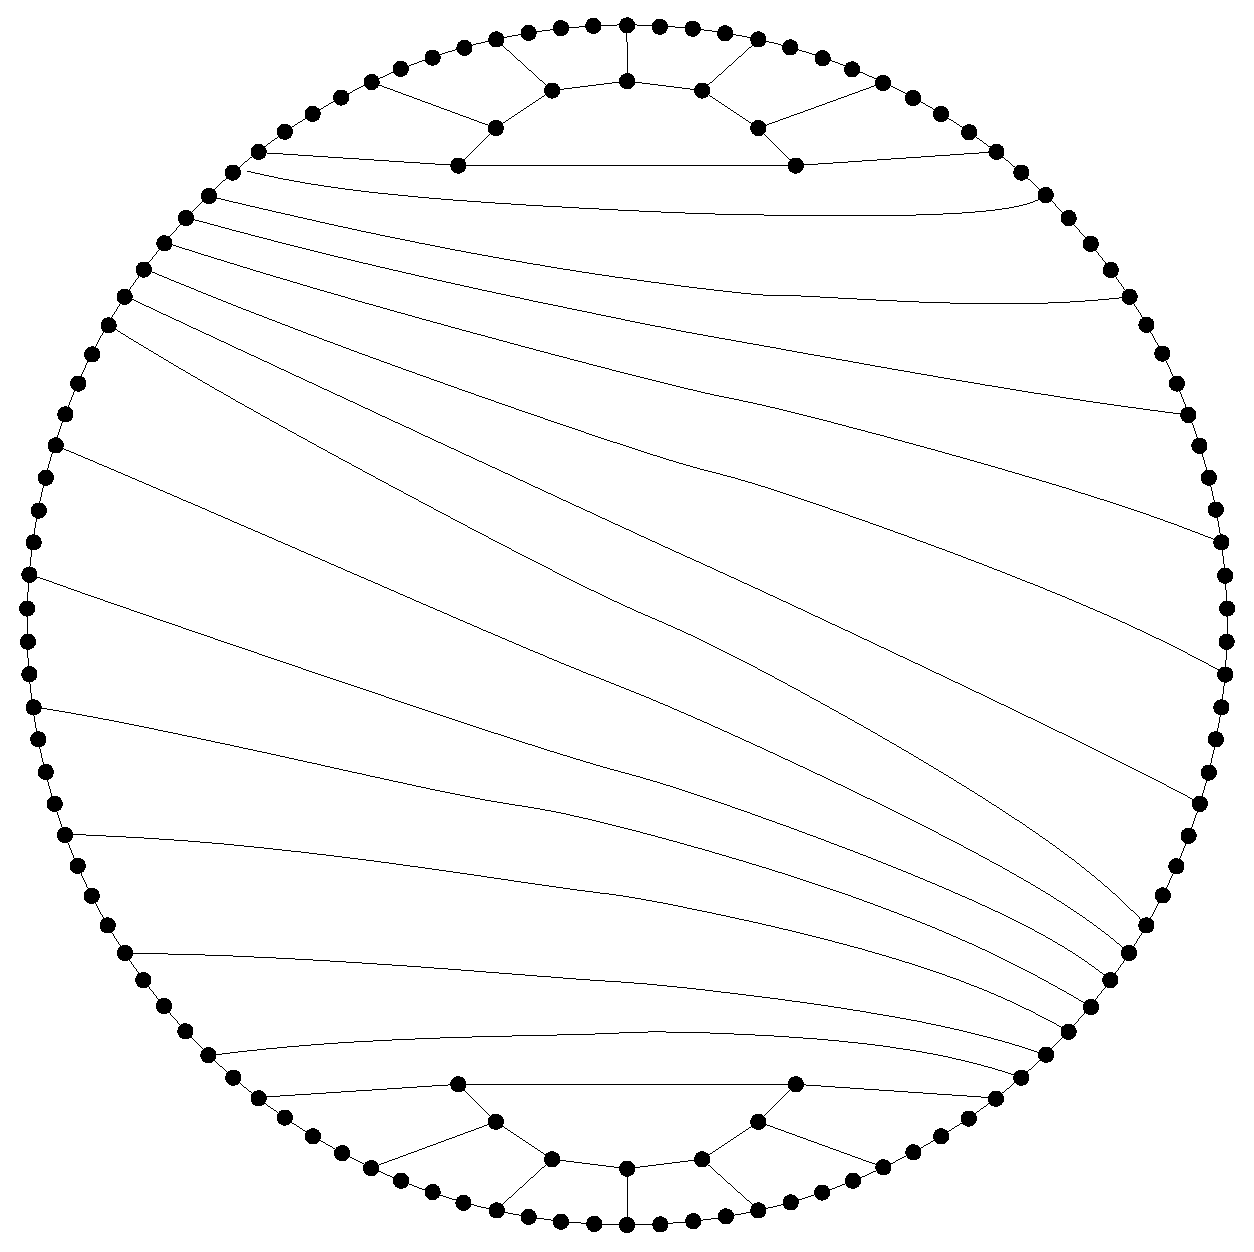
\epsfig{file=Boundary/HELICEN7gon.eps, width=5cm}\par
%Example: $(7,3)$-polycycle
\end{minipage}
\begin{minipage}{58mm}
\textcolor{red}{Boundary sequence} is:\\
$b=u2^{p-1}u3^{p-6}u2^{p-1}u3^{p-6}$\\
$u=(23^{p-4})^{p-1}2$;\\
$6p\hspace{-1mm}-\hspace{-1mm}2$ vertices of degree $3$ and\\
$4p^2\hspace{-1mm}-\hspace{-1mm}18p\hspace{-1mm}+\hspace{-1mm}4$ of degree $2$.\\
\\
\textcolor{red}{Symmetry groups} are:\\
of boundary: $C_{2v}$,\\
of polycycles: $C_2$.
\end{minipage}

\end{center}
This domain is filled in two ways (by $4p$ $p$-gons; $2p$ interior $3$-valent vertices).

\textcolor{red}{Thm.}: The boundary does not determine $(p,3)$-polycycle if $p\geq 5$.
\textcolor{red}{Conj.}: but it determines it if the filling is by less than $4p$ $p$-gons.



\end{slide}













\begin{slide}{Euler formula for $(p,3)$-polycycles}
Let $P$ be a $(p,3)$-polycycle.
Let $v_2$, $v_3$ be the number of vertices of degree $2$ or $3$ on the boundary.
Let $f_p$ the number of $p$-gonal faces and $x$ the number of interior vertices


{\it

{\bf Theorem}

(i) one has the relations

\begin{equation*}
\left\lbrace\begin{array}{rcl}
f_p-\frac{x}{2}&=&1+\frac{v_3}{2}\\
pf_p-3x        &=&v_2+2v_3
\end{array}\right.
\end{equation*}

(ii) If $p\not=6$, then $f_p$ and $x$ are determined by the boundary sequence.

(iii) If $p=6$, then $v_2=6+v_3$.
}

\end{slide}


\overlays{3}{
\begin{slide}{Possible filling}
\fromSlide{1}{Let us illustrate the algorithm for the simplest case $p=5$.\\
In some cases we can complete the patch directly.
}%
\onlySlide*{1}{
\vspace{1.5cm}
\begin{center}
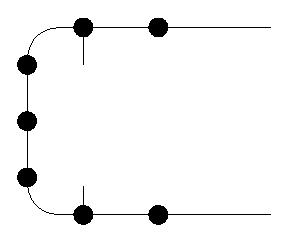
\epsfig{file=Boundary/ExampleAutoFill1.eps, width=4cm}\hspace{1cm}\epsfig{file=Boundary/ExampleAutoFill2.eps, width=4cm}
\end{center}
}%
\fromSlide{2}{
\vspace{1.5cm}
\begin{center}
\epsfig{file=Boundary/ExampleAutoFill1sec.eps, width=4cm}\hspace{1cm}\epsfig{file=Boundary/ExampleAutoFill2sec.eps, width=4cm}
\end{center}
}%
\fromSlide{3}{But in some cases more is needed:
\begin{center}
\epsfig{file=Boundary/DifficultCases.eps, width=4cm}
\end{center}
}
\end{slide}
}










\overlays{3}{
\begin{slide}{Different possible options}
\onlySlide*{1}{
\begin{minipage}{5cm}
\begin{center}
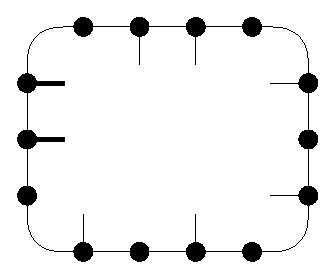
\epsfig{file=Boundary/IllustrationDifficult1.eps, width=4cm}
\end{center}
\end{minipage}
\begin{minipage}{5cm}
\begin{center}
\epsfig{file=Boundary/IllustrationDifficult6.eps, width=4cm}
\end{center}
\end{minipage}
}%
\onlySlide*{2}{
\begin{minipage}{5cm}
\begin{center}
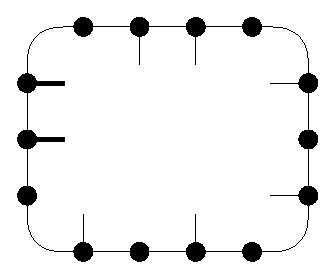
\epsfig{file=Boundary/IllustrationDifficult1.eps, width=4cm}
\end{center}
\end{minipage}
\newline
\begin{center}
%\begin{minipage}{10cm}
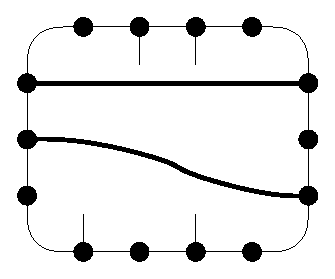
\epsfig{file=Boundary/IllustrationDifficult2.eps, width=4cm}\mbox{or}\epsfig{file=Boundary/IllustrationDifficult3.eps, width=4cm}
%\end{minipage}
\end{center}
}%
\onlySlide*{3}{
\begin{minipage}{5cm}
\begin{center}
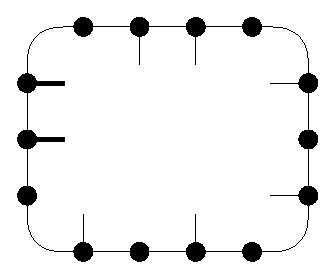
\epsfig{file=Boundary/IllustrationDifficult1.eps, width=4cm}
\end{center}
\end{minipage}
\newline
\begin{center}
%\begin{minipage}{10cm}
\epsfig{file=Boundary/IllustrationDifficult4.eps, width=4cm}\mbox{or}\epsfig{file=Boundary/IllustrationDifficult5.eps, width=4cm}
%\end{minipage}
\end{center}
}%
\end{slide}
}


\begin{slide}{Algorithm}

A \textcolor{red}{patch} of $p$-gonal faces is a group of faces with one or more boundaries.

Take a boundary of a patch of faces. Then:
\begin{enumerate}
\item Take a pair of vertices of degree $3$ on the boundary and consider all possible completions to form a $p$-gon.
\item Every possible case define another patch of faces. Depending on the choice, the patch will have one or more boundaries.
\item For any of those boundaries, reapply the algorithm.
\end{enumerate}
This algorithm is a tree search, since we consider all possible cases.

\end{slide}


\overlays{7}{
\begin{slide}{An example of a search}
\onlySlide*{1}{
\vspace{-2mm}
\begin{center}
\epsfig{file=Boundary/TreeSearch1bis.eps, width=7.8cm}
\end{center}
}%
\onlySlide*{2}{
\vspace{-2mm}
\begin{center}
\epsfig{file=Boundary/TreeSearch7.eps, width=7.8cm}
\end{center}
}%
\onlySlide*{3}{
\vspace{-2mm}
\begin{center}
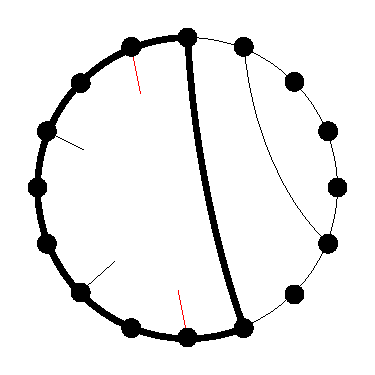
\epsfig{file=Boundary/TreeSearch8.eps, width=7.8cm}
\end{center}
}%
\onlySlide*{4}{
\vspace{-2mm}
\begin{center}
\epsfig{file=Boundary/TreeSearch9.eps, width=7.8cm}
\end{center}
}%
\onlySlide*{5}{
\vspace{-2mm}
\begin{center}
\epsfig{file=Boundary/TreeSearch10.eps, width=7.8cm}
\end{center}
}%
\onlySlide*{6}{
\vspace{-2mm}
\begin{center}
\epsfig{file=Boundary/TreeSearch11.eps, width=7.8cm}
\end{center}
}%
\onlySlide*{7}{
\vspace{-2mm}
\begin{center}
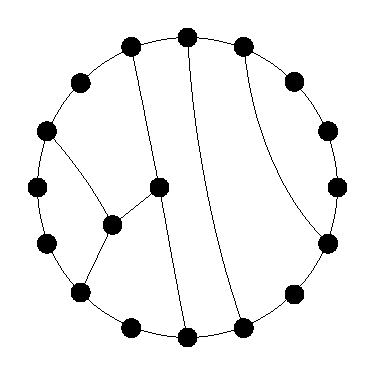
\epsfig{file=Boundary/TreeSearch12.eps, width=7.8cm}
\end{center}
}%

\end{slide}
}







\overlays{6}{
\begin{slide}{Another possible search}
\onlySlide*{1}{
\vspace{-2mm}
\begin{center}
\epsfig{file=Boundary/TreeSearch1.eps, width=7.8cm}
\end{center}
}%
\onlySlide*{2}{
\vspace{-2mm}
\begin{center}
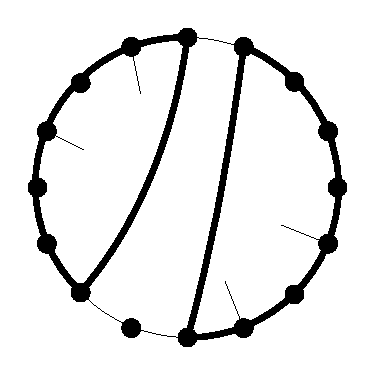
\epsfig{file=Boundary/TreeSearch2.eps, width=7.8cm}
\end{center}
}%
\onlySlide*{3}{
\vspace{-2mm}
\begin{center}
\epsfig{file=Boundary/TreeSearch3.eps, width=7.8cm}
\end{center}
}%
\onlySlide*{4}{
\vspace{-2mm}
\begin{center}
\epsfig{file=Boundary/TreeSearch4.eps, width=7.8cm}
\end{center}
}%
\onlySlide*{5}{
\vspace{-2mm}
\begin{center}
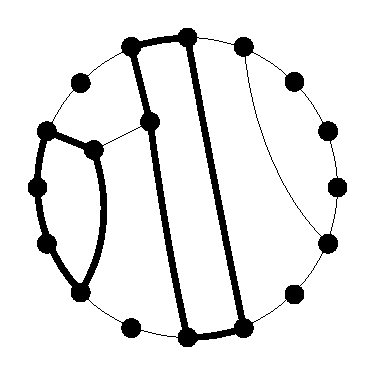
\epsfig{file=Boundary/TreeSearch5.eps, width=7.8cm}
\end{center}
}%
\onlySlide*{6}{
\vspace{-2mm}
\begin{center}
\epsfig{file=Boundary/TreeSearch6.eps, width=7.8cm}
\end{center}
}%

\end{slide}
}







\begin{slide}{Possible speedups}

\begin{itemize}
\item Limitation of tree size:
\begin{itemize}
\item Do all ``automatic fillings'' when there are some.
\item Then, we can select the pair of consecutive vertices of degree $3$ with maximal distance between them.
\end{itemize}
\item Kill some branches if :
\begin{itemize}
\item $f_p$ or $x$ are not non-negative integers (they are computed from the boundary sequence by Euler formula).
\item two consecutive vertices of degree $3$ do not admit any extension by a $p$-gon.
\end{itemize}
\end{itemize}
The combination of those tricks is insufficient in many cases.
For the enumeration of the maps $M_n(p,q)$ below, this is the critical bottleneck.


\end{slide}












\begin{slide}{}
\begin{center}
{\Huge 
\begin{tabular*}{8cm}{c}
\\[-0.5cm]
\textcolor{blue}{III. }\textcolor{red}{maps of $p$-gons}\\
\textcolor{red}{with a ring}
\textcolor{red}{of $q$-gons}
\end{tabular*}
}
\end{center}
\end{slide}





\begin{slide}{The problem}
A \textcolor{red}{$M_n(p,q)$} denotes a $3$-valent plane graph having only
$p$-gonal and $q$-gonal faces, such that the $q$-gonal faces form a \textcolor{red}{ring}, i.e. a simple cycle, of length $n$.

{\it
{\bf Theorem:} One has the equation
\begin{equation*}
((4-p)(q-4)+4)n+(6-p)(x+x')=4p
\end{equation*}
with $x$ and $x'$ being the number of interior vertices in two $(p,3)$-polycycles defines by the ring of $n$ $q$-gons.
}

\vspace{16mm}

{\scriptsize
M. Deza and V.P. Grishukhin, {\em  Maps of $p$-gons with a ring of $q$-gons},\\[-3mm]
Bull. of Institute of Combinatorics and its Applications {\bf 34} (2002) 99--110.
}
\end{slide}





%\textcolor{red}{$\Rightleftarrow$}

% $7$-gons are organized into



\begin{slide}{Classification theorem}
{\it 

{\bf Main Theorem}

Besides the cases $(p,q)$=$(7,5)$ and $(5,q)$ with $q\geq 8$, all such maps are known;
}


If $q=4$, then the map is $Prism_{p=n}$; from now, let $q\geq 5$.\\[2mm]

If $p=3$, two possibilities:
\begin{center}
\begin{minipage}{3cm}
\centering
\resizebox{2.6cm}{!}{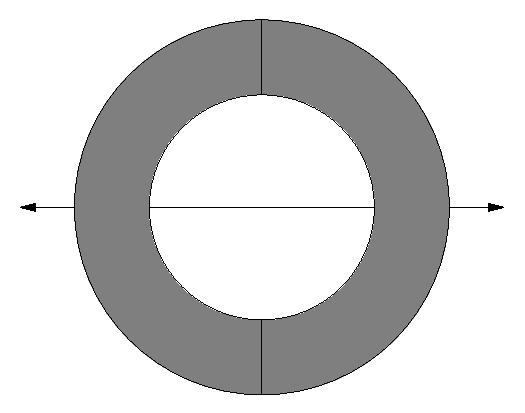
\includegraphics{Boundary/M2_3_6sec.eps}}\par
$M_{2}(3,6)(D_{2h})$
\end{minipage}
\begin{minipage}{3cm}
\centering
\resizebox{2.4cm}{!}{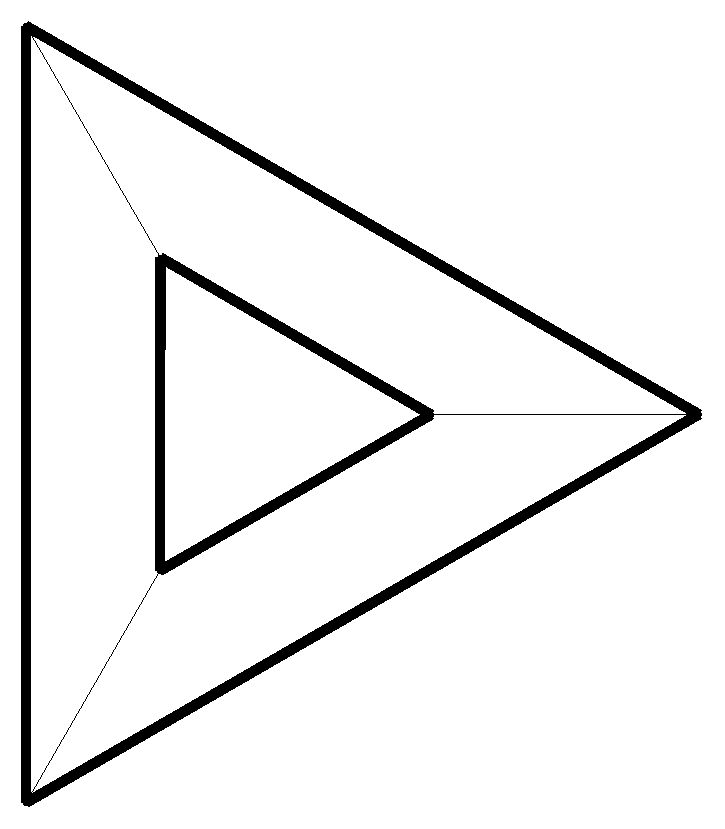
\includegraphics{Boundary/Prism3.eps}}\par
$M_{3}(3,4)(D_{3h})$
\end{minipage}
\end{center}


\end{slide}













\begin{slide}{Case $p=4$}

If $p=4$, two possibilities:

\begin{center}
\begin{minipage}{3cm}
\centering
\resizebox{2.4cm}{!}{\includegraphics{Boundary/M2_4_8.ps}}\par
$M_{2}(4,8)(D_{2h})$
\end{minipage}
\begin{minipage}{3cm}
\centering
\resizebox{2.4cm}{!}{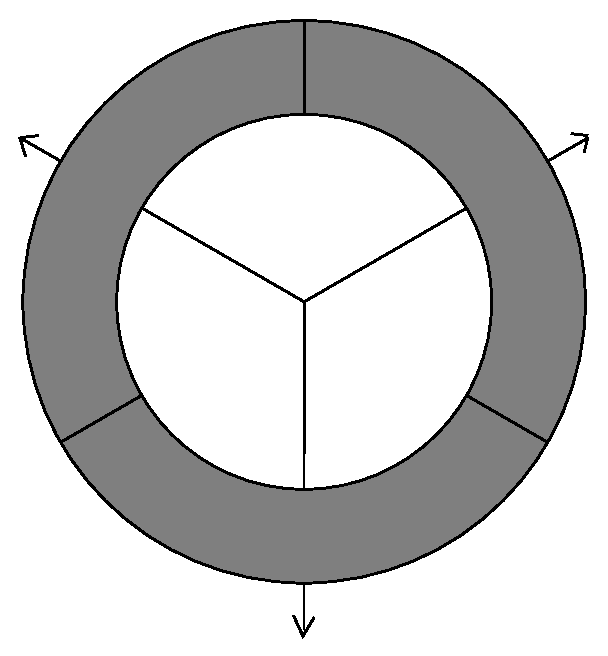
\includegraphics{Boundary/M3_4_6.ps}}\par
$M_{3}(4,6)(D_{3h})$
\end{minipage}
\end{center}
\textcolor{red}{and} an infinite serie\\[1mm]
\begin{center}
\begin{minipage}{2.6cm}
\centering
\resizebox{2.4cm}{!}{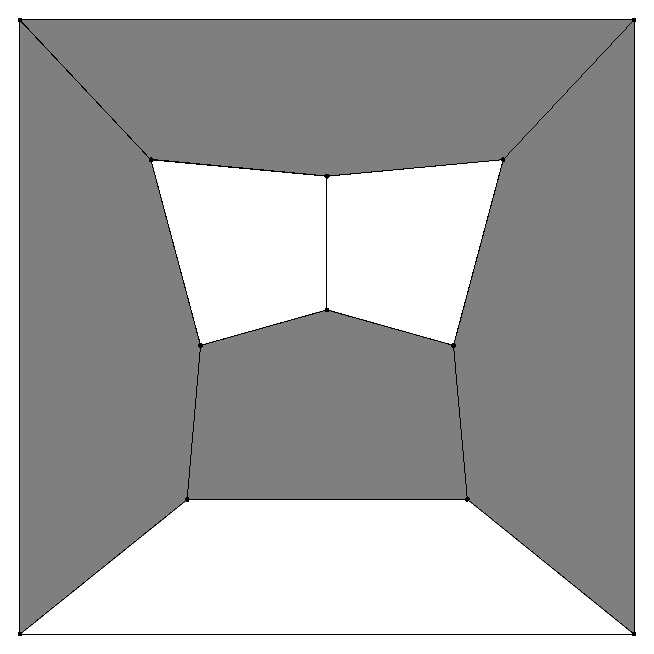
\includegraphics{Boundary/InfiniteStep5sec.eps}}\par
\end{minipage}
\begin{minipage}{2.6cm}
\centering
\resizebox{2.4cm}{!}{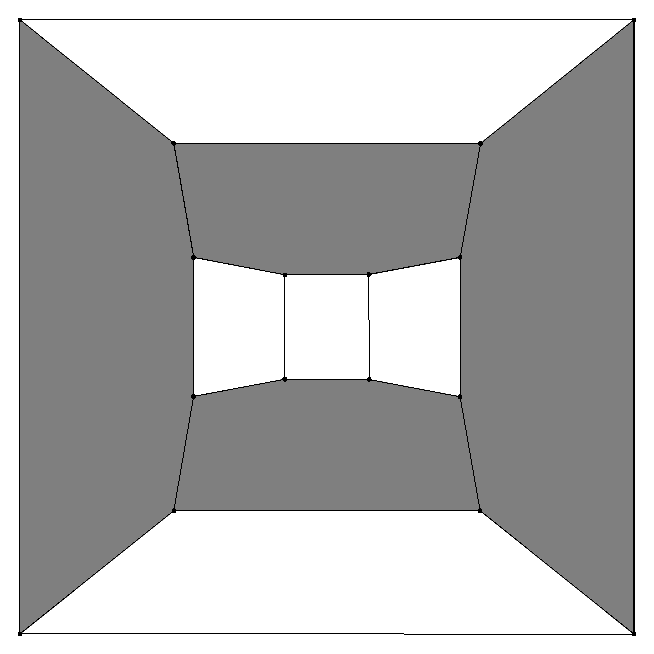
\includegraphics{Boundary/Infinite6-1sec.eps}}\par
\end{minipage}
\begin{minipage}{2.6cm}
\centering
\resizebox{2.6cm}{!}{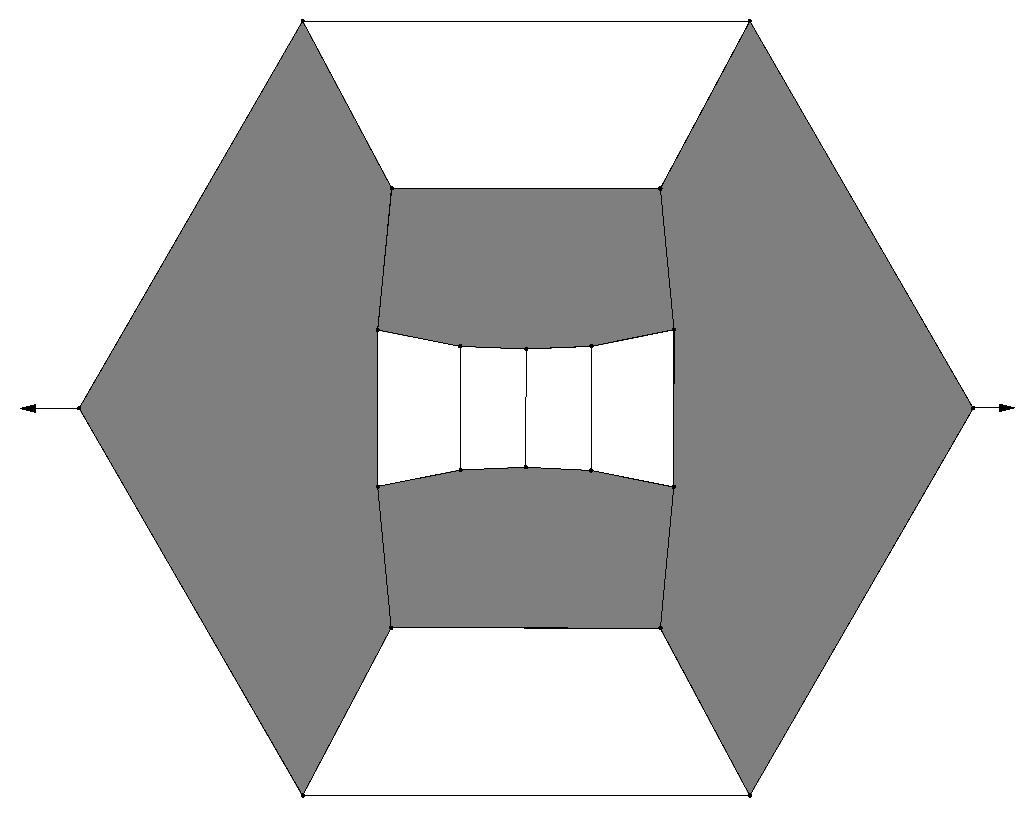
\includegraphics{Boundary/Infinite7-1this.eps}}\par
\end{minipage}
\begin{minipage}{2.6cm}
\centering
\resizebox{2.4cm}{!}{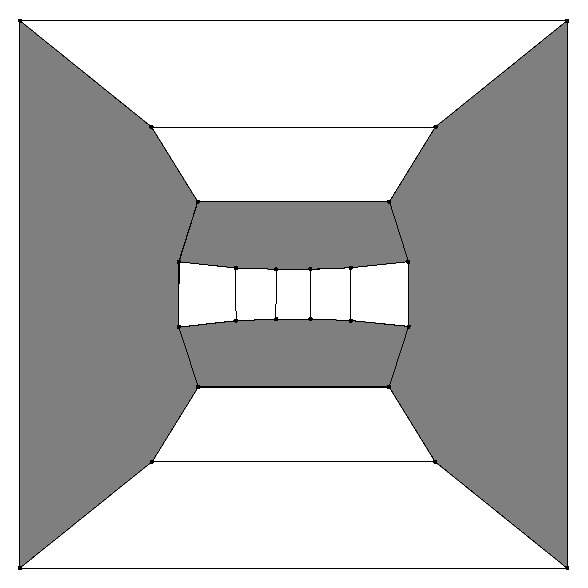
\includegraphics{Boundary/Infinite8-1sec.eps}}\par
\end{minipage}
\end{center}


\end{slide}











\begin{slide}{Case $p=5$}
\vspace{-4mm}
\begin{itemize}
\item If $q=5$, then this is Dodecahedron

\vspace{-1mm}

\item If $q=6$, then five possibilities:
\vspace{-1mm}
\begin{center}
\begin{minipage}{3.5cm}
\centering
\resizebox{2.2cm}{!}{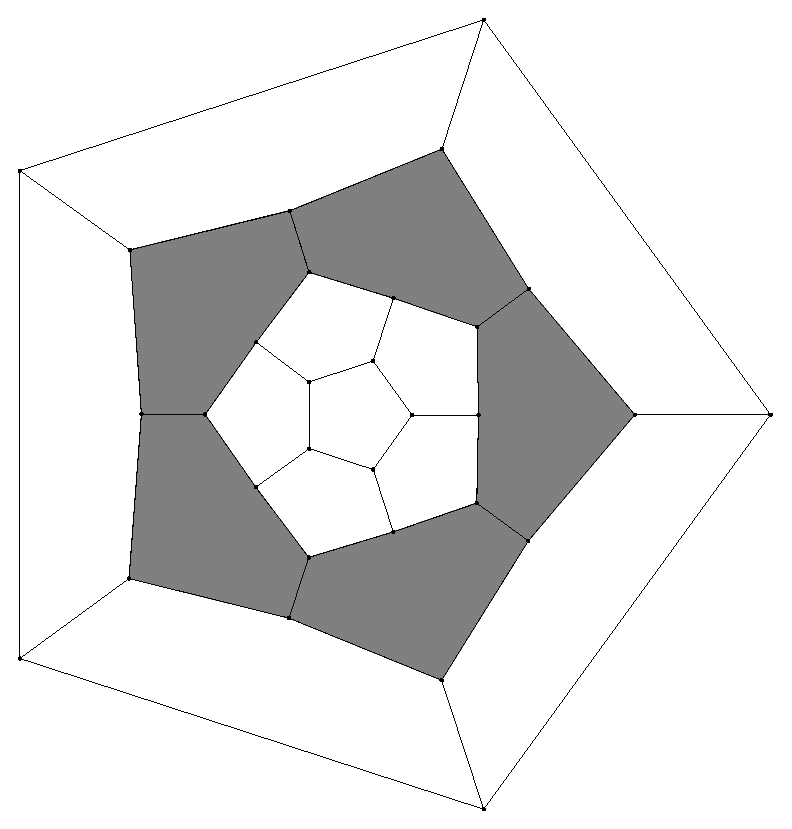
\includegraphics{Boundary/Graph56_1sec.eps}}\par
5, $D_{5h}$;6,6
\end{minipage}
\begin{minipage}{3.5cm}
\centering
\resizebox{2.2cm}{!}{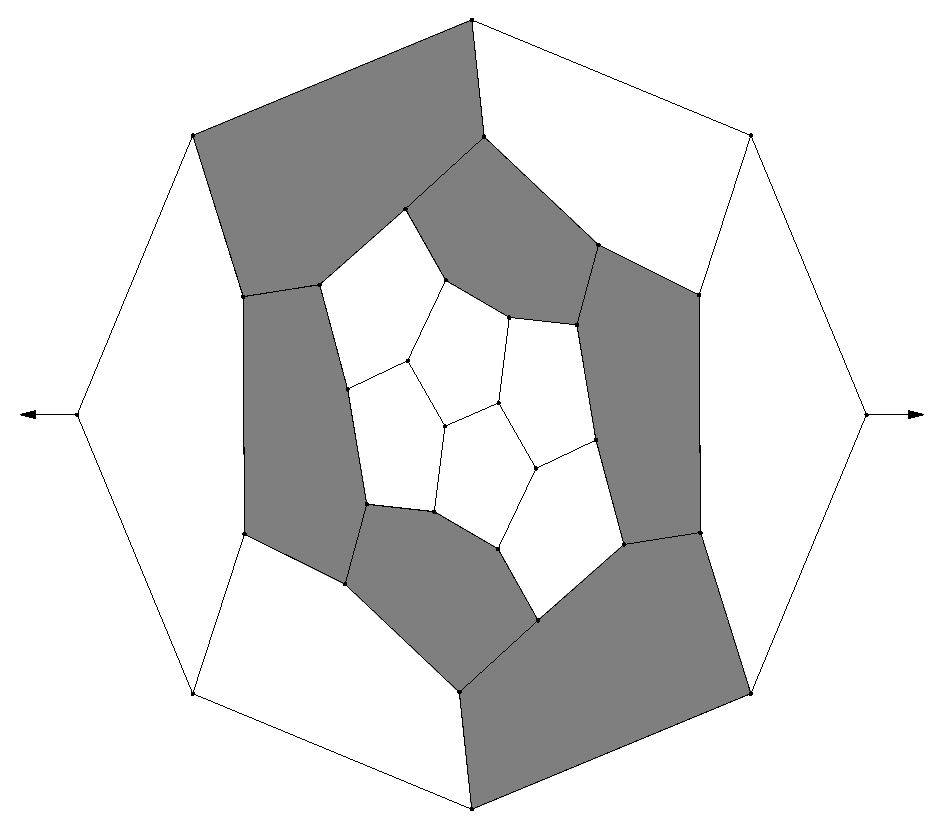
\includegraphics{Boundary/Graph56_2thi.eps}}\par
6, $D_2$;6,6
\end{minipage}
\begin{minipage}{3.5cm}
\centering
\resizebox{2.2cm}{!}{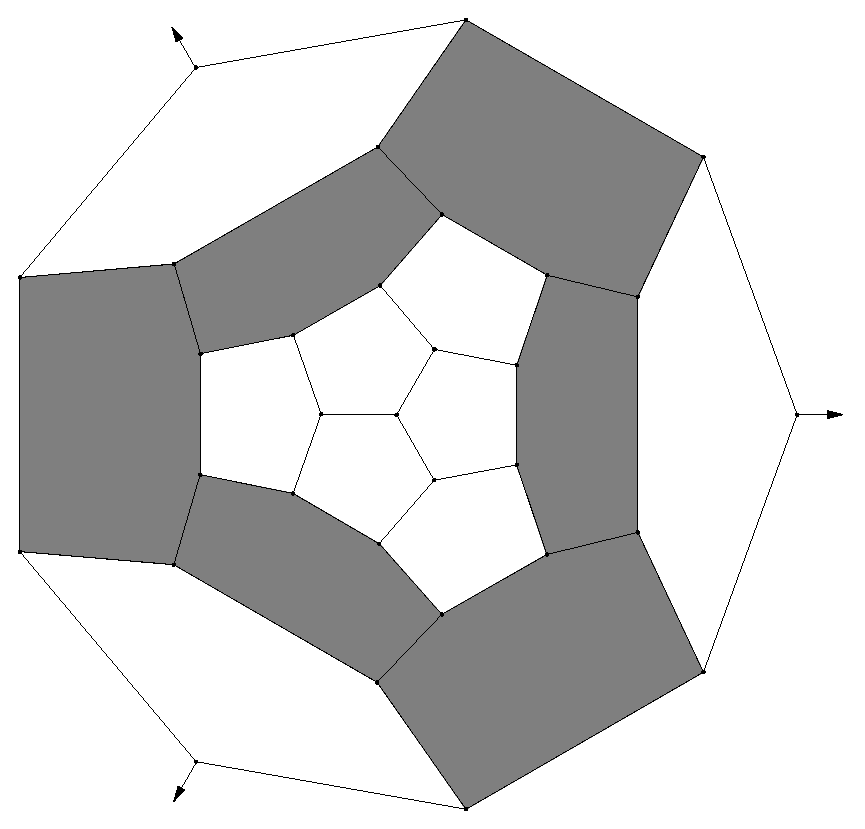
\includegraphics{Boundary/Graph56_3sec.eps}}\par
6, $D_{3d}$;6,6
\end{minipage}
\begin{minipage}{3.5cm}
\centering
\vspace{-3mm}
\resizebox{2.2cm}{!}{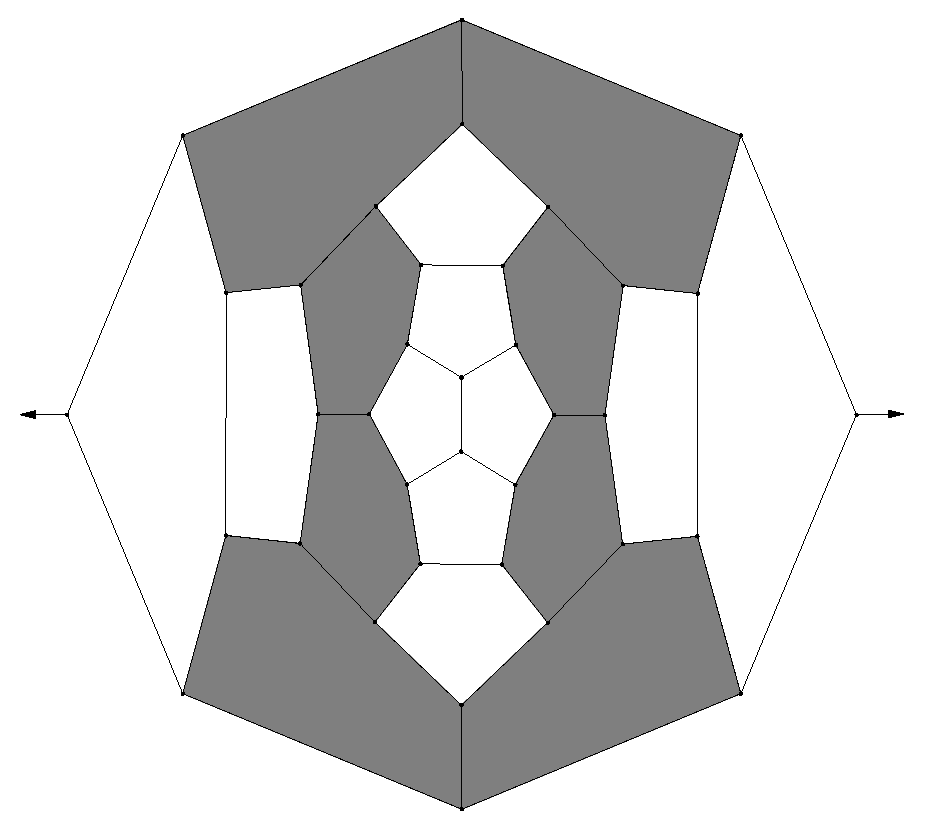
\includegraphics{Boundary/Graph56_4sec.eps}}\par
8, $D_{2d}$;6,6
\end{minipage}
\begin{minipage}{3.5cm}
\centering
\vspace{-3mm}
\resizebox{2.2cm}{!}{\includegraphics{Boundary/Graph56_5thi.eps}}\par
10, $D_2$;6,6
\end{minipage}
\end{center}

\item If $q=7$, then ten possibilities

\item If $q \ge 8$, we expect \textcolor{red}{infinity of possibilities}

\end{itemize}
\end{slide}




\begin{slide}{All $M_n(5,7)$}

\vspace{-5mm}
\begin{minipage}{3.7cm}
\centering
\epsfxsize=3.6cm
\epsffile{Boundary/Graph5_7_8-1newSec.eps}\par
4, $D_{2d}$;8,8
\end{minipage}
\begin{minipage}{3.7cm}
\centering
\epsfxsize=3.6cm
\epsffile{Boundary/Graph5_7_10newSec.eps}\par
10, $C_{2v}$;12,10
\end{minipage}
\hfill\begin{minipage}{3.7cm}
\centering
\epsfxsize=3.6cm
\epsffile{Boundary/Graph68-3_C2sec.eps}\par
12, $C_2$;10,14
\end{minipage}
\begin{minipage}{3.7cm}
\centering
\epsfxsize=3.1cm
\epsffile{Boundary/Graph68-4_C1sec.eps}\par
12, $C_1$;13,11
\end{minipage}
\begin{minipage}{3.7cm}
\centering
\epsfxsize=3.6cm
\epsffile{Boundary/Graph68-1_D2_thi.eps}\par
12, $D_2$;12,12
\end{minipage}
\hfill\begin{minipage}{3.7cm}
\centering
\epsfxsize=3.6cm
\epsffile{Boundary/Graph68-2_S4sec.eps}\par
12, $S_4$;12,12
\end{minipage}

\end{slide}





\begin{slide}{}
\begin{center}
\hspace{1cm}\begin{minipage}{3.5cm}
\centering
\epsfxsize=3.5cm
\epsffile{Boundary/Graph84-1_D2sec.eps}\par
16, $D_2$;14,14
\end{minipage}
\hfill\begin{minipage}{3.5cm}
\centering
\epsfxsize=3.5cm
\epsffile{Boundary/Graph84-2_D2thi.eps}\par
16, $D_2$;14,14
\end{minipage}\hspace{1cm}

\hspace{1cm}\begin{minipage}{3.5cm}
\centering
\epsfxsize=3.5cm
\epsffile{Boundary/Example20_1thi.eps}\par
20, $D_2$;16,16
\end{minipage}
\hfill\begin{minipage}{3.5cm}
\centering
\epsfxsize=3.5cm
\epsffile{Boundary/Example20_2thi.eps}\par
20, $C_2$;16,16
\end{minipage}\hspace{1cm}

\end{center}



\end{slide}






\begin{slide}{Case $p=6$}
If $p=6$, then $q=5$. There are four possibilities:

\begin{center}
\begin{minipage}{5cm}
\centering
\resizebox{3.0cm}{!}{\includegraphics{Boundary/Graph65_1thi.eps}}\par
12, $D_{2d}$;4,4
%????
\end{minipage}
\begin{minipage}{5cm}
\centering
\resizebox{3.0cm}{!}{\includegraphics{Boundary/Graph65_3thi.eps}}\par
12, $D_{3d}$;6,6
%?????
\end{minipage}
\begin{minipage}{5cm}
\centering
\resizebox{3.0cm}{!}{\includegraphics{Boundary/Graph65_4sec.eps}}\par
12, $D_{6d}$;7,7
%?????
\end{minipage}
\begin{minipage}{5cm}
\centering
\resizebox{3.0cm}{!}{\includegraphics{Boundary/Graph65_2thi.eps}}\par
12, $D_2$;6,6
%?????
\end{minipage}



\end{center}

\end{slide}




\begin{slide}{Two remaining undecided cases}
\vspace{-3.5mm}
If $p=7$, then $q=5$ and $n-(x+x')=28$. Two examples:
\begin{center}
\begin{minipage}{5cm}
\centering
\resizebox{4.3cm}{!}{\includegraphics{Boundary/Graph7_5_8-1newSec.eps}}\par
28, $D_2$;8,8
\end{minipage}
\begin{minipage}{5cm}
\centering
\resizebox{4cm}{!}{\includegraphics{Boundary/Graph7_5_9-1newSec.eps}}\par
30, $D_3$;9,9
\end{minipage}
\end{center}

The remaining undecided case is $M_n(5,q)$ with $q\geq 8$.

\begin{itemize}
\item Hadjuk and Sot\'ak found an infinity of maps $M_n(7,5)$,
\item Madaras and Sot\'ak found infinity of maps $M_n(5,q)$ for $q=10$ and $q\equiv 2,3\pmod 5$, $q\geq 8$.
\end{itemize}


\end{slide}






\begin{slide}{Enumeration techniques}
\vspace{-3mm}
\begin{itemize}
\item Harmuth enumerated all $3$-valent plane graphs with at most $84$ vertices, faces of gonality $5$ or $7$ and such that every faces of gonality $7$ is adjacent to two faces of gonality $7$ (i.e. $7$-gons are organised into disjoint simple cycles).
It gives all $M_{n}(5,7)$ with $n\leq 16$.
\item Remaining case $17\leq n\leq 20$ is treated by following algorithm:
\begin{center}
\begin{minipage}{3.5cm}
\centering
\resizebox{30mm}{!}{\includegraphics{Boundary/Completion3.eps}}\par
Generating patches
\end{minipage}
\begin{minipage}{3.5cm}
\centering
\resizebox{30mm}{!}{\includegraphics{Boundary/Completion2.eps}}\par
Adding ring of $q$ gons
\end{minipage}
\begin{minipage}{3.5cm}
\centering
\resizebox{30mm}{!}{\includegraphics{Boundary/Completion1.eps}}\par
completing (if possible).
\end{minipage}
\end{center}


\end{itemize}

\end{slide}












\begin{slide}{Known $M_n(5,8)$}

\vspace{-5mm}
\begin{minipage}{3.7cm}
\centering
\resizebox{3.07cm}{!}{\includegraphics{Boundary/Graph5_8_9-1newSec.eps}}\par
3, $D_{3h}$;9,9
\end{minipage}
\begin{minipage}{3.7cm}
\centering
\resizebox{3.5cm}{!}{\includegraphics{Boundary/Graph5_8_10-3newSec.eps}}\par
4, $D_{2d}$;10,10
\end{minipage}
\hfill\begin{minipage}{3.7cm}
\centering
\resizebox{3.5cm}{!}{\includegraphics{Boundary/Graph5_8_10-2newSec.eps}}\par
8, $C_2$;10,18
\end{minipage}
\begin{minipage}{3.7cm}
\centering
\resizebox{3.2cm}{!}{\includegraphics{Boundary/Graph5_8_11-1newSec.eps}}\par
9, $C_s$;19,11
\end{minipage}
\begin{minipage}{3.7cm}
\centering
\resizebox{3.7cm}{!}{\includegraphics{Boundary/Graph5_8_10-4newSec.eps}}\par
10, $C_{2v}$;10,22
\end{minipage}
\hfill\begin{minipage}{3.7cm}
\centering
\resizebox{3.7cm}{!}{\includegraphics{Boundary/Graph5_8_14-5newSec.eps}}\par
10, $C_2$;14,18
\end{minipage}
\end{slide}













\begin{slide}{}

\vspace{-7mm}
\begin{minipage}{3.7cm}
\centering
\resizebox{3.07cm}{!}{\includegraphics{Boundary/Graph5_8_14-2newSec.eps}}\par
11, $C_1$;20,14
\end{minipage}
\begin{minipage}{3.7cm}
\centering
\resizebox{3.5cm}{!}{\includegraphics{Boundary/Graph5_8_10-1newSec.eps}}\par
12, $C_2$;26,10
\end{minipage}
\hfill\begin{minipage}{3.7cm}
\centering
\resizebox{3.5cm}{!}{\includegraphics{Boundary/Graph5_8_14-1newSec.eps}}\par
12, $C_2$;14,22
\end{minipage}
\begin{minipage}{3.7cm}
\centering
\resizebox{3.7cm}{!}{\includegraphics{Boundary/Graph5_8_14-4newSec.eps}}\par
12, $C_2$;14,22
\end{minipage}
\begin{minipage}{3.7cm}
\centering
\resizebox{3.4cm}{!}{\includegraphics{Boundary/Graph5_8_15-1newSec.eps}}\par
12, $C_1$;21,15
\end{minipage}
\hfill\begin{minipage}{3.7cm}
\centering
\resizebox{3.4cm}{!}{\includegraphics{Boundary/Graph5_8_15-2newSec.eps}}\par
13, $C_1$;15,23
\end{minipage}
\end{slide}




\begin{slide}{}
\vspace{-8mm}
\begin{center}
\hspace{1cm}\begin{minipage}{3.5cm}
\centering
\resizebox{3.7cm}{!}{\includegraphics{Boundary/Graph5_8_12-1newSec.eps}}\par
14, $C_2$;28,12
\end{minipage}
\hfill\begin{minipage}{3.5cm}
\centering
\resizebox{3.3cm}{!}{\includegraphics{Boundary/Graph5_8_14-3newSec.eps}}\par
16, $C_1$;30,14
\end{minipage}\hspace{1cm}

\hspace{1cm}\begin{minipage}{3.5cm}
\centering
\resizebox{3.6cm}{!}{\includegraphics{Boundary/Graph5_8_14-6newSec.eps}}\par
18, $C_2$;14,34
\end{minipage}
\hfill\begin{minipage}{3.5cm}
\centering
\resizebox{3.5cm}{!}{\includegraphics{Boundary/Graph5_8_15-3newSec.eps}}\par
18, $C_3$;33,15
\end{minipage}\hspace{1cm}

\end{center}

\end{slide}










\begin{slide}{Known $M_n(5,9)$}
\vspace{-6mm}
\begin{minipage}{5cm}
\centering
\resizebox{3.9cm}{!}{\includegraphics{Boundary/Graph5_9_10-3newSec.eps}}\par
6, $C_2$;10,20
\end{minipage}
\hfill\begin{minipage}{5cm}
\centering
\resizebox{3.9cm}{!}{\includegraphics{Boundary/Graph5_9_8-2newSec.eps}}\par
10, $C_2$;34,8
\end{minipage}
\begin{minipage}{5cm}
\vspace{-1mm}
\centering
\resizebox{3.7cm}{!}{\includegraphics{Boundary/Graph5_9_8-1newSec.eps}}\par
12, $C_2$;40,8
\end{minipage}
\hfill\begin{minipage}{5cm}
\vspace{-1mm}
\centering
\resizebox{3.7cm}{!}{\includegraphics{Boundary/Graph5_9_9-1newSec.eps}}\par
12, $C_3$;39,9
\end{minipage}
\end{slide}









\begin{slide}{}
\vspace{-9mm}
\begin{center}

\begin{minipage}{5cm}
\centering
\resizebox{4.3cm}{!}{\includegraphics{Boundary/Graph5_9_10-1newSec.eps}}\par
12, $C_2$;38,10
\end{minipage}
\hfill\begin{minipage}{5cm}
\centering
\resizebox{4cm}{!}{\includegraphics{Boundary/Graph5_9_10-4newSec.eps}}\par
12, $C_2$;38,10
\end{minipage}
\begin{minipage}{5cm}
\centering
\vspace{-8mm}
\resizebox{4cm}{!}{\includegraphics{Boundary/Graph5_9_10-2newSec.eps}}\par
12, $C_1$;38,10
\end{minipage}
\end{center}
\end{slide}



%\begin{slide}{Known $M_n(5,10)$}
%
%\begin{minipage}{5cm}
%\centering
%\resizebox{4cm}{!}{\includegraphics{Boundary/M2_5_10.ps}}\par
%\end{minipage}
%
%\end{slide}


\begin{slide}{Known $M_{n}(5,10)$}
\vspace{-5mm}
\begin{center}
\begin{minipage}{36mm}
\centering
\resizebox{32mm}{!}{\includegraphics{Boundary/Graph5_10_10-2newSec.eps}}\par
2, $D_{2h}$;10,10
\end{minipage}
\begin{minipage}{36mm}
\centering
\resizebox{35mm}{!}{\includegraphics{Boundary/WeakAzul510_one_cycle1thi.eps}}\par
6, $C_2$;12,24
\end{minipage}
\hfill\begin{minipage}{36mm}
\centering
\resizebox{35mm}{!}{\includegraphics{Boundary/WeakAzul510_one_cycle2thi.eps}}\par
6, $C_{2v}$;14,22
\end{minipage}
\begin{minipage}{36mm}
\centering
\resizebox{32mm}{!}{\includegraphics{Boundary/WeakAzul510_one_cycle3sec.eps}}\par
6, $C_s$;13,23
\end{minipage}
\begin{minipage}{36mm}
\centering
\resizebox{35mm}{!}{\includegraphics{Boundary/WeakAzul510_one_cycle4thi.eps}}\par
6, $C_2$;14,22
\end{minipage}
\hfill\begin{minipage}{36mm}
\centering
\resizebox{35mm}{!}{\includegraphics{Boundary/WeakAzul510_one_cycle5thi.eps}}\par
6, $C_{2v}$;12,24
\end{minipage}
%\begin{minipage}{62mm}
%\centering
%\resizebox{56mm}{!}{\rotatebox{90}{\includegraphics{Boundary/Graph5_10_10-1newSec.eps}}}\par
%14, $C_2$;58,10
%\end{minipage}
\end{center}

\end{slide}





\begin{slide}{}
\vspace{-8mm}
\begin{minipage}{36mm}
\centering
\resizebox{33mm}{!}{\includegraphics{Boundary/WeakAzul510_one_cycle6sec.eps}}\par
6, $C_1$;15,21
\end{minipage}
\begin{minipage}{36mm}
\centering
\resizebox{33mm}{!}{\includegraphics{Boundary/Graph5_10_11-3sec.eps}}\par
12, $C_1$;11,49
\end{minipage}
\hfill\begin{minipage}{36mm}
\centering
\resizebox{35mm}{!}{\includegraphics{Boundary/Graph5_10_10-1newSec.eps}}\par
14, $C_2$;58,10
\end{minipage}
\begin{minipage}{36mm}
\centering
\resizebox{33mm}{!}{\includegraphics{Boundary/Graph5_10_11-1sec.eps}}\par
14, $C_1$;11,57
\end{minipage}
\begin{minipage}{36mm}
\centering
\resizebox{33mm}{!}{\includegraphics{Boundary/Graph5_10_11-2sec.eps}}\par
14, $C_1$;11,57
\end{minipage}
\hfill\begin{minipage}{36mm}
\centering
\resizebox{33mm}{!}{\includegraphics{Boundary/Graph5_10_11-4sec.eps}}\par
14, $C_1$;11,57
\end{minipage}





%\begin{minipage}{5cm}
%\centering
%\resizebox{3.5cm}{!}{\includegraphics{Graph5_10_11-1sec.eps}}\par
%14, $C_1$;11,57
%\end{minipage}
%\hfill\begin{minipage}{5cm}
%\centering
%\resizebox{3.5cm}{!}{\includegraphics{Graph5_10_11-2sec.eps}}\par
%14, $C_1$;11,57
%\end{minipage}
%\begin{minipage}{5cm}
%\centering
%\resizebox{3.5cm}{!}{\includegraphics{Boundary/Graph5_10_11-3sec.eps}}\par
%12, $C_1$;11,49
%\end{minipage}
%\hfill\begin{minipage}{5cm}
%\centering
%\resizebox{3.5cm}{!}{\includegraphics{Boundary/Graph5_10_11-4sec.eps}}\par
%14, $C_1$;11,57
%\end{minipage}



\end{slide}









\begin{slide}{All parameters $(p,q)$}



\begin{minipage}{50mm}
\begin{center}
{\scriptsize
\begin{tabular}{||c|c|c||}
\hline
\hline
$(p,q)$       &$n$        &maps\\
\hline
$(p\geq 3,4)$ &$p$        &$1(Prism_p)$\\
$(3,6)$       &$2$        &$1$\\
\hline
$(4,5)$       &$4$        &$1$\\
$(4,6)$       &$3,4$      &$2$\\
$(4,7)$       &$4$        &$1$\\
$(4,8)$       &$2,4$      &$2$\\
$(4,q>8)$     &$4$        &$1$\\
\hline
$(6,5)$       &$12$       &$4$(full.)\\
\hline
\hline
\end{tabular}
}
\end{center}
\end{minipage}
\begin{minipage}{55mm}
\begin{center}
{\scriptsize
\begin{tabular}{||c|c|c||}
\hline
\hline
$(p,q)$       &$n$        &maps\\
\hline
$(5,5)$       &$5,6$      &$3$(Dode.)\\
$(5,6)$       &$5, 6, 8,10$           &$5$(full.)\\
$(5,7)$       &$4, 10, 12, 16, 20$  &$10$(azu.)\\
$(5,8)$       &$\geq 3$   &\textcolor{red}{$\geq 16$}\\
$(5,9)$       &$\geq 6$   &\textcolor{red}{$\geq 7$}\\
$(5,10)$      &$\geq 2$   &\textcolor{red}{$\geq 2$}\\
$(5,q> 10)$   &$\geq 2$   &\textcolor{red}{?}\\
\hline
$(7,5)$       &$\geq 28$  &\textcolor{red}{$\geq 2$}(azu.)\\
\hline
\hline
\end{tabular}
}
\end{center}
\end{minipage}


\end{slide}



\begin{slide}{}
\begin{center}
{\Huge 
\begin{tabular*}{8cm}{c}
\\[-0.5cm]
\textcolor{blue}{IV. }\textcolor{red}{Generalizations}\\
\end{tabular*}
}
\end{center}
\end{slide}




\begin{slide}{Several rings}
A \textcolor{red}{$M_{n_1,\dots, n_t}(p,q)$} denotes a $3$-valent plane graph with $p$-gons and $q$-gons, where $q$-gons form $t$ rings of length $n_1$, \dots, $n_t$ (equiv. each $q$-gon is adjacent exactly to two $q$-gons).

{\it

{\bf Theorem}: One has the equation
\begin{equation*}
(4-(4-p)(4-q))\sum_i n_i+(6-p)(\textcolor{red}{x_1}+\textcolor{red}{x_2})=4p, \mbox{,~{\em where}}
\end{equation*}
\begin{itemize}
\item \textcolor{red}{$x_1$} is the number of vertices incident to $3$ $p$-gonal faces and
\item \textcolor{red}{$x_2$} the number of vertices incident to $3$ $q$-gonal faces.
\end{itemize}

}
\begin{itemize}
\item[\ding{224}] \textcolor{red}{finiteness} for $(4,q)$, $(5,6)$, $(5,7)$ but we have \textcolor{red}{infinity} for $(6,5)$ and, possibly, for $(5,q)$, $q\geq 8$.


\end{itemize}

\end{slide}






\begin{slide}{The case $(p,q)$=$(5,6)$ (fullerenes)}

All maps \textcolor{red}{$M_{\dots}(5,6)$} are:
\begin{itemize}
\item five maps with one ring of $6$-gons,
\item following three maps with two rings of $6$-gons:
\begin{center}
\begin{minipage}{35mm}
\centering
\resizebox{33mm}{!}{\rotatebox{0}{\includegraphics{Boundary/Graph32_5thi.eps}}}\par
%\resizebox{33mm}{!}{\rotatebox{0}{\includegraphics{Boundary/Graph32_54th.eps}}}\par
$D_{3h}$; 32
\end{minipage}
\begin{minipage}{35mm}
\centering
\resizebox{33mm}{!}{\rotatebox{0}{\includegraphics{Boundary/Graph38_16thi.eps}}}\par
%\resizebox{33mm}{!}{\rotatebox{0}{\includegraphics{Boundary/Graph38_164th.eps}}}\par
$C_{3v}$; 38
\end{minipage}
\begin{minipage}{35mm}
\centering
\resizebox{38mm}{!}{\rotatebox{90}{\includegraphics{Boundary/Graph40_39sec.eps}}}\par
%\resizebox{33mm}{!}{\rotatebox{90}{\includegraphics{Boundary/Graph40_39sec.eps}}}\par
$D_{5h}$; 40
\end{minipage}
\end{center}

\end{itemize}


\end{slide}





\begin{slide}{\textcolor{red}{Two} rings of $7$-gons filled by $5$-gons}

\vspace{-7mm}
\begin{center}
\begin{minipage}{37mm}
\centering
\resizebox{35mm}{!}{\rotatebox{0}{\includegraphics{Boundary/Incorrect5_7_01thi.eps}}}\par
$C_{2h}$; 44
\end{minipage}
\begin{minipage}{37mm}
\centering
\resizebox{35mm}{!}{\rotatebox{0}{\includegraphics{Boundary/Incorrect5_7_02thi.eps}}}\par
$D_3$; 44
\end{minipage}
\begin{minipage}{37mm}
\centering
\resizebox{35mm}{!}{\rotatebox{0}{\includegraphics{Boundary/Incorrect5_7_03sec.eps}}}\par
$D_{5d}$; 60
\end{minipage}
\begin{minipage}{37mm}
\centering
\resizebox{35mm}{!}{\rotatebox{0}{\includegraphics{Boundary/Incorrect5_7_04sec.eps}}}\par
$D_{5h}$; 60
\end{minipage}
\begin{minipage}{37mm}
\centering
\resizebox{35mm}{!}{\rotatebox{0}{\includegraphics{Boundary/Incorrect5_7_08thi.eps}}}\par
$D_{3d}$; 68
\end{minipage}
\begin{minipage}{37mm}
\centering
\resizebox{35mm}{!}{\rotatebox{0}{\includegraphics{Boundary/Incorrect5_7_11thi.eps}}}\par
$D_3$; 68
\end{minipage}
\end{center}





%\begin{minipage}{37mm}
%\centering
%\resizebox{35mm}{!}{\rotatebox{90}{\includegraphics{Boundary/Incorrect5_7_01sec.eps}}}\par
%$C_{2h}$; 44
%\end{minipage}
%\begin{minipage}{37mm}
%\centering
%\resizebox{35mm}{!}{\rotatebox{90}{\includegraphics{Boundary/Incorrect5_7_02sec.eps}}}\par
%$D_3$; 44
%\end{minipage}
%\begin{minipage}{37mm}
%\centering
%\resizebox{35mm}{!}{\rotatebox{90}{\includegraphics{Boundary/Incorrect5_7_03sec.eps}}}\par
%$D_{5d}$; 60
%\end{minipage}
%\begin{minipage}{37mm}
%\centering
%\resizebox{35mm}{!}{\rotatebox{90}{\includegraphics{Boundary/Incorrect5_7_04sec.eps}}}\par
%$D_{5h}$; 60
%\end{minipage}
%\begin{minipage}{37mm}
%\centering
%\resizebox{35mm}{!}{\rotatebox{90}{\includegraphics{Boundary/Incorrect5_7_08sec.eps}}}\par
%$D_{3d}$; 68
%\end{minipage}
%\begin{minipage}{37mm}
%\centering
%\resizebox{35mm}{!}{\rotatebox{90}{\includegraphics{Boundary/Incorrect5_7_11sec.eps}}}\par
%$D_3$; 68
%\end{minipage}

\end{slide}







\begin{slide}{\textcolor{red}{Two} rings of $7$-gons filled by $5$-gons}
\vspace{-7mm}
\begin{center}
\begin{minipage}{37mm}
\centering
\resizebox{35mm}{!}{\rotatebox{0}{\includegraphics{Boundary/Incorrect5_7_06thi.eps}}}\par
$D_2$; 68
\end{minipage}
\begin{minipage}{37mm}
\centering
\resizebox{35mm}{!}{\rotatebox{0}{\includegraphics{Boundary/Incorrect5_7_07thi.eps}}}\par
$D_2$; 68
\end{minipage}
\begin{minipage}{37mm}
\centering
\resizebox{35mm}{!}{\rotatebox{0}{\includegraphics{Boundary/Incorrect5_7_09thi.eps}}}\par
$D_2$; 68
\end{minipage}
\begin{minipage}{37mm}
\centering
\resizebox{35mm}{!}{\rotatebox{0}{\includegraphics{Boundary/Incorrect5_7_10thi.eps}}}\par
$D_2$; 68
\end{minipage}
\begin{minipage}{37mm}
\centering
\resizebox{35mm}{!}{\rotatebox{0}{\includegraphics{Boundary/Incorrect5_7_13thi.eps}}}\par
$C_{2h}$; 76
\end{minipage}
\begin{minipage}{37mm}
\centering
\resizebox{35mm}{!}{\rotatebox{0}{\includegraphics{Boundary/Incorrect5_7_05thi.eps}}}\par
$T$; 68
\end{minipage}
\end{center}


%\begin{center}
%\begin{minipage}{37mm}
%\centering
%\resizebox{35mm}{!}{\rotatebox{90}{\includegraphics{Boundary/Incorrect5_7_06sec.eps}}}\par
%$D_2$; 68
%\end{minipage}
%\begin{minipage}{37mm}
%\centering
%\resizebox{35mm}{!}{\rotatebox{90}{\includegraphics{Boundary/Incorrect5_7_07sec.eps}}}\par
%$D_2$; 68
%\end{minipage}
%\begin{minipage}{37mm}
%\centering
%\resizebox{35mm}{!}{\rotatebox{90}{\includegraphics{Boundary/Incorrect5_7_09sec.eps}}}\par
%$D_2$; 68
%\end{minipage}
%\begin{minipage}{37mm}
%\centering
%\resizebox{35mm}{!}{\rotatebox{90}{\includegraphics{Boundary/Incorrect5_7_10sec.eps}}}\par
%$D_2$; 68
%\end{minipage}
%\begin{minipage}{37mm}
%\centering
%\resizebox{35mm}{!}{\rotatebox{90}{\includegraphics{Boundary/Incorrect5_7_12sec.eps}}}\par
%$C_{2v}$; 76
%\end{minipage}
%\begin{minipage}{37mm}
%\centering
%\resizebox{35mm}{!}{\rotatebox{90}{\includegraphics{Boundary/Incorrect5_7_14sec.eps}}}\par
%$C_{3v}$; 80
%\end{minipage}
%\end{center}



\end{slide}








\begin{slide}{Remaining graphs $M_{\dots}(5,7)$ (azulenoids)}
%The case $(p,q)$=$(5,7)$ (azulenoids)

\vspace{-7mm}
\begin{center}
\begin{minipage}{37mm}
\centering
\resizebox{35mm}{!}{\rotatebox{0}{\includegraphics{Boundary/Incorrect5_7_12thi.eps}}}\par
$C_{2v}$; 76
\end{minipage}
\begin{minipage}{37mm}
\centering
\resizebox{35mm}{!}{\rotatebox{0}{\includegraphics{Boundary/Incorrect5_7_14thi.eps}}}\par
$C_{3v}$; 80
\end{minipage}
\begin{minipage}{37mm}
\centering
\resizebox{35mm}{!}{\rotatebox{0}{\includegraphics{Boundary/Incorrect5_7_16thi.eps}}}\par
$C_{3v}$; 92
\end{minipage}
\begin{minipage}{37mm}
\centering
\resizebox{35mm}{!}{\rotatebox{0}{\includegraphics{Boundary/Incorrect5_7_15sec.eps}}}\par
$D_{5d}$; 100
\end{minipage}
\end{center}




%\begin{center}
%\begin{minipage}{47mm}
%\centering
%\resizebox{40mm}{!}{\rotatebox{90}{\includegraphics{Boundary/Incorrect5_7_13sec.eps}}}\par
%$C_{2h}$; 76
%\end{minipage}
%\begin{minipage}{47mm}
%\centering
%\resizebox{40mm}{!}{\rotatebox{90}{\includegraphics{Boundary/Incorrect5_7_05sec.eps}}}\par
%$T$; 68
%\end{minipage}
%\end{center}
%
%All $3$-valent maps of $5$- and $7$-gons ($7$-gons forming disjoint simple rings) with at most $84$ vertices are (T.Harmuth):
%\begin{itemize}
%\item $8$, $12$ with one, two rings, respectively,
%\item $1$, $1$ with three, four rings, respectively.
%\end{itemize}
%Undecided cases are: $88$, $92$, $96$, $100$ vertices only.



\end{slide}





\begin{slide}{The case $(p,q)$=\textcolor{red}{$(6,5)$} (fullerenes)}

All maps \textcolor{red}{$M_{\dots}(6,5)$} are:
\begin{itemize}
\item four maps with exactly one ring of $5$-gons,
\item the maps:

\begin{center}
\begin{minipage}{3.5cm}
\centering
\resizebox{35mm}{!}{\rotatebox{0}{\includegraphics{Boundary/Graph38_16_7th.eps}}}\par
special map
\end{minipage}
\begin{minipage}{3.5cm}
\centering
\resizebox{35mm}{!}{\rotatebox{0}{\includegraphics{Boundary/Graph40_40sec.eps}}}\par
infinite family: $4$ triples of pentagons
\end{minipage}
\begin{minipage}{3.5cm}
\centering
\resizebox{35mm}{!}{\rotatebox{0}{\includegraphics{Boundary/Graph36_15sec.eps}}}\par
infinite family:
$t\geq 1$ concentric
$6$-rings of hexagons
\end{minipage}
\end{center}

\end{itemize}

\end{slide}




\overlays{4}{
\begin{slide}{Infinite families}
\fromSlide{1}{
For any $t\geq 0$, there exists a map $M_{3,\dots,3}(5,8)$ (with $t$ $3$-rings of $8$-gons) and a map $M_{2,\dots,2}(5,10)$ (with $t$ $2$-rings of $10$-gons)
}%
\onlySlide*{1}{
\begin{center}
\begin{minipage}{4.5cm}
\centering
\resizebox{40mm}{!}{\rotatebox{0}{\includegraphics{Boundary/Serie58_1sec.eps}}}\par
\end{minipage}
\begin{minipage}{4.5cm}
\centering
\resizebox{40mm}{!}{\rotatebox{0}{\includegraphics{Boundary/Serie510_1sec.eps}}}\par
\end{minipage}
\end{center}
}%
\onlySlide*{2}{
\begin{center}
\begin{minipage}{4.5cm}
\centering
\resizebox{40mm}{!}{\rotatebox{0}{\includegraphics{Boundary/Serie58_2sec.eps}}}\par
\end{minipage}
\begin{minipage}{4.5cm}
\centering
\resizebox{40mm}{!}{\rotatebox{0}{\includegraphics{Boundary/Serie510_2sec.eps}}}\par
\end{minipage}
\end{center}
}%
\onlySlide*{3}{
\begin{center}
\begin{minipage}{4.5cm}
\centering
\resizebox{40mm}{!}{\rotatebox{0}{\includegraphics{Boundary/Serie58_3sec.eps}}}\par
\end{minipage}
\begin{minipage}{4.5cm}
\centering
\resizebox{40mm}{!}{\rotatebox{0}{\includegraphics{Boundary/Serie510_3sec.eps}}}\par
\end{minipage}
\end{center}
}%
\onlySlide*{4}{
\begin{center}
\begin{minipage}{4.5cm}
\centering
\resizebox{40mm}{!}{\rotatebox{0}{\includegraphics{Boundary/Serie58_4sec.eps}}}\par
\end{minipage}
\begin{minipage}{4.5cm}
\centering
\resizebox{40mm}{!}{\rotatebox{0}{\includegraphics{Boundary/Serie510_4sec.eps}}}\par
\end{minipage}
\end{center}
}%

\end{slide}
}



\begin{slide}{\textcolor{red}{$k$}-valent maps}
A \textcolor{red}{$M^k_n(p,q)$} denotes a \textcolor{red}{$k$}-valent map with $p$-gons and $q$-gons only, where $q$-gons form a ring of length $n$.

\begin{itemize}
\item The only $M^4_{n}(p,3)$ is $p$-gonal antiprism.
\item All $M^4_n(3,4)$ are:
\begin{center}
\begin{minipage}{2.6cm}
\centering
\epsfxsize=2.2cm
\epsffile{Boundary/8-hedrite10_2secBAND.eps}\par
$D_{4h}$; 10
\end{minipage}
\begin{minipage}{2.6cm}
\centering
\epsfxsize=2.2cm
\epsffile{Boundary/8-hedrite12-5sec.eps}\par
$D_{3d}$; 12
\end{minipage}
\begin{minipage}{2.6cm}
\centering
\epsfxsize=2.2cm
\epsffile{Boundary/8Hedrite12_2_4th.eps}\par
$D_{2}$; 12
\end{minipage}
\begin{minipage}{2.6cm}
\centering
\epsfxsize=2.2cm
\epsffile{Boundary/DecoratedRhombiDodecahedronSec.eps}\par
$D_{2d}$; 14
\end{minipage}
\end{center}
There is only one other \textcolor{red}{$M^4_{\dots}(3,4)$}; it has two rings of $4$-gons, $14$ vertices and symmetry $D_{4h}$.


\end{itemize}



\end{slide}












\end{document}
